\documentclass[10pt,letterpaper]{article} % {{{
\usepackage[top=0.85in,left=2.75in,footskip=0.75in]{geometry}
\usepackage{amsmath,amssymb}
% Use adjustwidth environment to exceed column width (see example table in text)
\usepackage{changepage}

% textcomp cpackage and marvosym package for additional characters
\usepackage{textcomp,marvosym}
\usepackage{subcaption}


\usepackage[T1]{fontenc}
\usepackage{lmodern}
% cite package, to clean up citations in the main text. Do not remove.
\usepackage{cite}

% Use nameref to cite supporting information files (see Supporting Information section for more info)
\usepackage{nameref,hyperref}

% line numbers
\usepackage[right]{lineno}

% ligatures disabled
\usepackage[nopatch=eqnum]{microtype}
\DisableLigatures[f]{encoding = *, family = * }

% color can be used to apply background shading to table cells only
\usepackage[table]{xcolor}

% array package and thick rules for tables
\usepackage{array}
\usepackage{caption}
\captionsetup[figure]{labelfont={bf},labelformat={default},labelsep=period,name={Fig}}


% create "+" rule type for thick vertical lines
\newcolumntype{+}{!{\vrule width 2pt}}

% create \thickcline for thick horizontal lines of variable length
\newlength\savedwidth
\newcommand\thickcline[1]{%
  \noalign{\global\savedwidth\arrayrulewidth\global\arrayrulewidth 2pt}%
  \cline{#1}%
  \noalign{\vskip\arrayrulewidth}%
  \noalign{\global\arrayrulewidth\savedwidth}%
}

% \thickhline command for thick horizontal lines that span the table
\newcommand\thickhline{\noalign{\global\savedwidth\arrayrulewidth\global\arrayrulewidth 2pt}%
\hline
\noalign{\global\arrayrulewidth\savedwidth}}


% Remove comment for double spacing
%\usepackage{setspace} 
%\doublespacing

% Text layout
\raggedright
\setlength{\parindent}{0.5cm}
\textwidth 5.25in 
\textheight 8.75in

% Bold the 'Figure #' in the caption and separate it from the title/caption with a period
% Captions will be left justified
\usepackage[aboveskip=1pt,labelfont=bf,labelsep=period,justification=raggedright,singlelinecheck=off]{caption}
\renewcommand{\figurename}{Fig}
\renewcommand{\succ}{\textrm{succ}}

\newcommand{\fref}[1]{Fig~\ref{#1}}
\newcommand{\eref}[1]{Eq~(\ref{#1})}
% Use the PLoS provided BiBTeX style
\bibliographystyle{plos2015}

% Remove brackets from numbering in List of References
\makeatletter
\renewcommand{\@biblabel}[1]{\quad#1.}
\makeatother



% Header and Footer with logo
\usepackage{lastpage,fancyhdr,graphicx}
\usepackage{epstopdf}



\usepackage[english]{babel}
\usepackage{graphicx,helvet}
\usepackage{color}
\usepackage{url}
\usepackage{amssymb}
\usepackage[utf8]{inputenc}
\usepackage{hyperref}
% \usepackage[inline]{showlabels}
\usepackage{bbm,bm}
\usepackage{soul}
\usepackage{amsfonts}

\usepackage{tikz}
\usetikzlibrary{arrows}
\usetikzlibrary{quantikz}

\usepackage[draft,inline,nomargin]{fixme} \fxsetup{theme=color}
\FXRegisterAuthor{cp}{acp}{\color{blue}CP}
\FXRegisterAuthor{tb}{ttb}{\color{green}TB}




%\pagestyle{myheadings}
\pagestyle{fancy}
\fancyhf{}
%\setlength{\headheight}{27.023pt}
\rfoot{\thepage/\pageref{LastPage}}
\renewcommand{\headrulewidth}{0pt}
\renewcommand{\footrule}{\hrule height 2pt \vspace{2mm}}
\fancyheadoffset[L]{2.25in}
\fancyfootoffset[L]{2.25in}
\lfoot{\today}

%% Include all macros below

\newcommand{\lorem}{{\bf LOREM}}
\newcommand{\ipsum}{{\bf IPSUM}}
\DeclareMathOperator{\tr}{tr}
\newtheorem{definition}{Definition}
\newtheorem{theorem}{Theorem}

%% END MACROS SECTION

% }}}
\begin{document}

\section{Simulación de cosas de dos qubits}

En general, un canal de dos qubits va a requerir 4 qubits de ancilla. El circuito para hacerlo es una de las figuras del artículo y es una generalización sencilla del de un qubit.\\

Algunos posibles canales a simular son por ejemplo:
\begin{itemize}
\item $\varepsilon(\rho) = k \rho + (1-k) (\sigma_z \otimes \sigma_z) \rho (\sigma_z \otimes \sigma_z) $.
\item $\varepsilon(\rho) = (1-k_1-k_2) \rho + k_1 (\sigma_z \otimes I) \rho (\sigma_z \otimes I) + k_2 (I \otimes \sigma_z) \rho (I \otimes \sigma_3)$.
\end{itemize}
Como el primer canal solo involucra 2 de los 16 operadores de Pauli, en realidad sólo requiere un qubit de ancilla. El segundo canal requiere 2 qubits de ancilla. \\

Entonces, los dos son fáciles de implementar en las compus cuánticas. 
Por ejemplo, el segundo canal se puede hacer con el siguiente circuito:

\begin{figure}[h!]
\begin{quantikz}
\lstick{$q_0$} & \qw  & \gate{\sigma_3} & \qw & \qw  \\
\lstick{$q_1$} & \qw & \qw & \gate{\sigma_3}  & \qw  \\
\lstick{$\tilde{q}_0$} & \gate[wires=2][3cm]{\quad\quad \text{Crear el estado de dos qubits}\quad\quad} & \octrl{-2} & \ctrl{-1}  & \qw \\
\lstick{$\tilde{q}_1$} & \gateinput{$\;\;\;\;\;\;\; \sqrt{1-k_1-k_2} |0 \rangle |0 \rangle + \sqrt{k_1} |0 \rangle |1 \rangle + \sqrt{k_2} |1 \rangle |0 \rangle $} & \ctrl{-3} & \octrl{-2} & \qw
\end{quantikz}
\end{figure}

Por ejemplo, para unos cuantos puntos dentro de las opciones de $k_1, k_2$ para el segundo canal, se obtienen las siguientes fidelidades:

\begin{figure}[h!]
\begin{center}
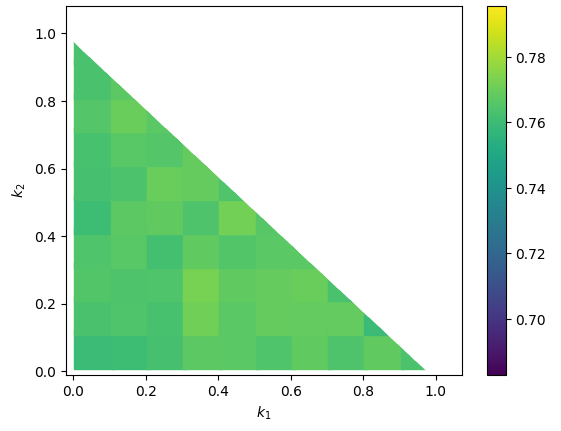
\includegraphics[width=0.5\textwidth]{images/2qbit.png}\\
\caption{Fidelidades para distintas elecciones de $k_1, k_2$ para el segundo canal mostrado arriba.  Al parecer las fidelidades no cambian mucho. }
\end{center}
\end{figure}

\newpage
\section{Ver cómo suben los datos otros artículos similares de Plos One}

Por lo que encontré, muchos de los artículos no tenían datos abiertos al público.
De los pocos que sí, casi todos subían un link a un repositorio de github que  contiene el código que hayan usado y quizá documentos con los resultados de dicho código.\\

Puse lo que pienso que se podría subir en la carpeta "Codigo/Para_subir" en el repositorio. 




\section{Revisar la motivación que ponen otras simulaciones cuánticas}

Algunos artículos que encontré y lo que ponen:

\begin{itemize}
\item \textbf{Efficient universal quantum channel simulation in IBM's cloud quantum computer (Shi-Jie Wei, Tao Xin, Gui-Lu long) Science China:}\\ 

Quantum simulation can efficiently simulate the dynamics of diverse systems
[1, 6-10] in condensed matter [11, 12], quantum chemistry
[13], and high-energy physics [14-16], which are intractable
by classical computers. Moreover, every practical quantum
system is open system because of the inevitable coupling to
the environment. Thus, quantum simulation of open system
is an equally important and more general subject to explore.
However, open system quantum simulation is still in the
early stages of development [17-23] and remains largely unexplored. The quantum simulation of open systems promises
powerful applications in a class of physical problems, such as
preparing various special state [24-28], thermalizing in spinboson systems and complex many fermion-boson systems
[29, 30], and studying nonequilibrium dynamics [31]. \\

\item \textbf{Testing quantum computers with the protocl of quantum state matching (Adrian Ortega, Orsolya Kalman) Physica Scripta} \\

The fields of Quantum Computation and Quantum Information have received a huge boost in the last years with
the advent of ‘public’ quantum computation. Current devices can be accessed remotely, opening the possibility
for the larger public to carry out experiments and to test them by running programs. Quantum computers(qcs)
can be based on several different physical systems such as superconducting qubits[1–3], trapped ions[4],
photonic devices[5] and neutral atoms[6]. Given all these possibilities, questions, such as computational
efficiency, error correction capability, stability and computational power start to become important matters for
future applications.\\

\item \textbf{Experimental quantum channel simulation (He Lu et al)}: \\

Quantum simulation [1–3] is the most promising near-term
application of quantum computing due to the resource requirements for imitating some classically intractable systems
being significantly less onerous that for other applications
such as factorization. Experimental quantum simulation on
closed systems is well studied using photons [4], atoms [5]
and trapped ions [6]. Quantum simulation of open-system
dynamics also has variety of applications, such as dissipative quantum phase transitions [7] and dissipative quantumstate engineering [8], thermalization [9], quantum noise generators [10], non-Markovian dynamics [11], and non-unitary
quantum computing [12].

\item  \textbf{Optimizing Parametrized Quantum Circuits
with Free-Axis Single-Qubit Gates (Hiroshi Watanabe)}:\\

Parametrized quantum circuit (PQC) is one of the most essential components of hybrid quantum-classical
algorithms on near-term quantum devices [1–3]. \\

The design of PQC is critical in variational quantum algorithms. Oversimplified PQC cannot express
the optimal quantum state even if it could be implemented on noisy quantum devices. On the other
hand, a PQC designed with a deep circuit for high expressibility cannot be implemented on currently available noisy quantum devices.\\

\item \textbf{Simulating noisy quantum channels via quantum state preparation algorithms (Marcelo Zanetti et al):} \\

En este artículo hacen un algoritmo para simular canales cuánticos generales y lo demuestran en las computadoras de IBM. Sin embargo, no hablan mucho de motivación. 

\item \textbf{Single-qubit rotations in parametrized quantum circuits (S. E. Rasmussen, Loft)}:\\

En éste ven cómo optimizar algoritmos cuánticos parametrizados reduciendo la cantidad de rotaciones de un qubit.

\item \textbf{Experimental Implementation of Quantum Walks on
IBM Quantum Computers (F. Acasiete et al.)}

\item \textbf{Experimental Demonstration of Force Driven Quantum Harmonic Oscillator in IBM
Quantum Computer (Alakesh Baishya et al.)} \\

Quantum simulation is one of the tremendously growing areas in the field of quantum computation which
has significant goals and opportunities1
. From the
past decades, this powerful area has been applied to
variety of scientific disciplines, e.g., physics2–6, quantum chemistry7,8, quantum biology9,10, and computer
science11 to name a few. Several time-dependent mass
harmonic oscillators including the most famous socalled Caldirola-Kanai oscillator12,13 have been extensively studied over the past years14–17. IBM quantum
experience, has played a considerable role from the recent years, the platform using which a number of research
works have been performed in the field of quantum simulation. These include observation of Uhlmann phase19
,
chemical isomerization reaction20, simulation of far-fromequilibrium dynamics21, Ising model simulation22, quantum multi-particle tunneling23, quantum scrambling24
,
and simulation of Klein-Gordon equation25 to name a
few. Other sub-disciplines such as developing quantum
algorithms26–33, testing of quantum information theoretical tasks34–38, quantum cryptography39–42, quantum error correction43–46, quantum applications47–52 have also
been explored.


\item  \textbf{Quantum amplitude estimation algorithms on IBM quantum
devices (Pooja Rao et al)}

\item  \textbf{Classical simulation of intermediate-size quantum circuits (Jianxin Chen et al.)}


Classically simulating quantum systems is a relatively old problem [1]. However, only recently have nascent
quantum computers become competitive in simulating general quantum circuits. Recent announcements of larger
systems with reasonable target fidelities [2, 3] are pushing the boundary of what classical simulations can handle.
With this push, a variety of techniques have been invented in order to keep up with newer quantum processors
[4–11]. Unfortunately, this race is one that us classical beings cannot win in the long-term, but there are many good
reasons to try. \\

\item \textbf{Quantum circuit simulation of superchannels (Kai Wang and Dong-Sheng Wang)} \\

In modern quantum physics, the control and engineering of complex quantum dynamics is essential. In
recent years, quantum computing has become a powerful paradigm to achieve this. With the standard
quantum circuit model, the field of digital quantum simulation is expected to be powerful to realize and
study quantum dynamics






\end{itemize}




\section{La definicion de circuito cuantico}

En ningún lugar se define bien qué es un circuito cuántico. Por ejemplo, en wikipedia lo definen así:

In quantum information theory, a quantum circuit is a model for quantum computation, similar to classical circuits, in which a computation is a sequence of quantum gates, measurements, initializations of qubits to known values, and possibly other actions.


\end{document}
